\section{力}\label{sec:2-1}

在日常生活和生产劳动中,我们经常要用力。当我们用手推车、拉锯、提水桶、压木板的时候,都要用力。
用力的时候,就会感到肌肉紧张。因此,人类对力的认识,最初是从肌肉紧张的感觉中得来的。

推车、拉锯、提水桶、压木板的时侯,人用了力,物体(车、锯、水桶、木板)就受到了力。
通常我们就把对物体的推、拉、提、压等作用叫做力的作用。

不仅人能对物体施加力,一个物体对别的物体也能施加力。
例如,推土机推土的时候,推土机对土就施加了力。
拖拉机拉犁的时候,拖拉机对犁就施加了力。
起重机吊起货物的时候,起重机对货物就施加了力。
压路机压路的时候,压路机对路就施加了力,等等。

彼此不直接接触的物体之间,也能发生力的作用。
例如,让磁铁靠近铁钉,在磁铁还没有挨着铁钉的时候,就能把铁钉吸起来(图 \ref{fig:2-1}),表明磁铁对铁钉施加了力。
用摩擦带电的塑料棒靠近碎纸片,在塑料棒还没有挨着纸片的时候,就能把碎纸片吸起来(图 \ref{fig:2-2}),表明塑料棒对纸片施加了力。

\begin{figure}[htbp]
    \centering
    \begin{minipage}{7cm}
    \centering
    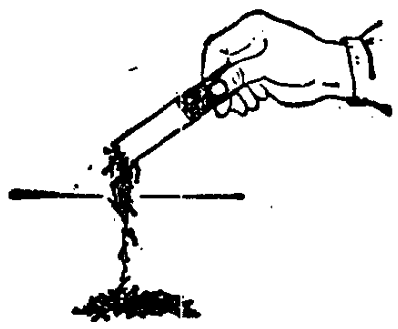
\includegraphics[width=6cm]{../pic/czwl1-ch2-1}
    \caption{磁铁吸引铁钉}\label{fig:2-1}
    \end{minipage}
    \qquad
    \begin{minipage}{7cm}
    \vspace{1.5cm}%图片向下显示,以便 caption 能大致在同一水平线
    \centering
    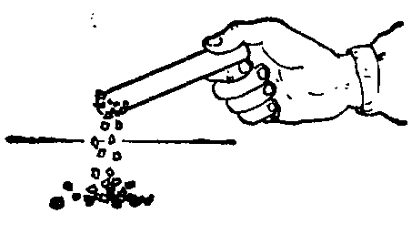
\includegraphics[width=6cm]{../pic/czwl1-ch2-2}
    \caption{带电的塑料棒吸引碎纸片}\label{fig:2-2}
    \end{minipage}
\end{figure}

从这些例子中可以看出,\textbf{力是物体对物体的作用}。
一个物体受到了力,一定有另一个物体对它施加这种作用。
没有物体,就不会有力的作用。

推车的时候,人用了力,车受到了力,我们就说人是施力物体,车是受力物体。
物体间发生力的作用时,一定有施力物体和受力物体。
在一个物体受到施力物体的力的作用时,为了简便起见,我们通常只说物体受到了力,而不特别指明施力物体。
但是必须知道,施力物体是一定存在的。

\begin{figure}[htbp]
    \centering
    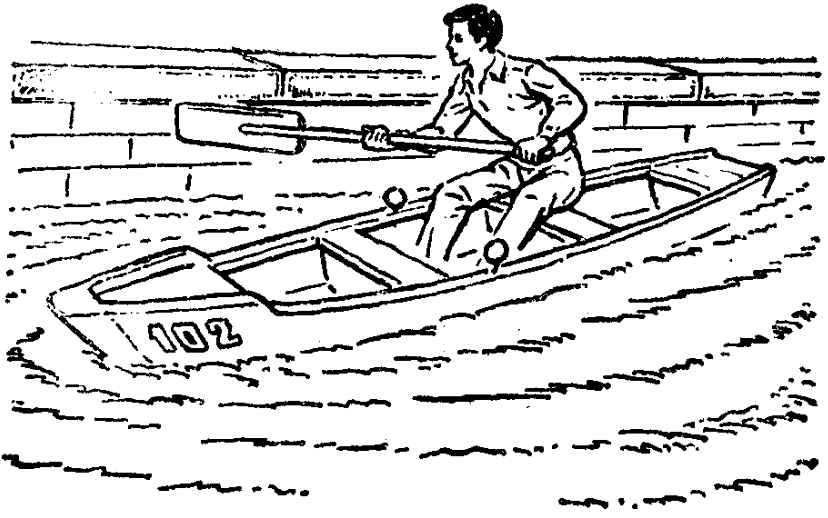
\includegraphics[width=0.6\textwidth]{../pic/czwl1-ch2-3}
    \caption{}\label{fig:2-3}
\end{figure}

我们提水桶的时候,会感到手也受到水桶的向下的拉力。
可见,不但手对水桶施加了力,同时水桶对手也施加了力。
坐在船上的人用力推岸时,船就会离岸而去(图 \ref{fig:2-3}),表明人和船同时也受到了岸的推力。
这些现象表明,\textbf{物体间力的作用是相互的}。
就是说,一个物体对另一个物体施力时,同时也受到另一个物体对它的力的作用。
反之,一个物体受到另一个物体对它的力的作用时,同时它也对另一个物体施加力的作用。


